%%%%%%%%%%%%%%%%%%%%%%%%%%%%%%%%%%%%%%%%%%%%%%%%%%%%%%%%%%%%%%%%%%%%%%%
\chapter{Textual Editing Framework - TEF}
With TEF it is possible to integrate textual editing in an existing MVC editor. This is done by selecting an element, showing its textual representation in an extra overlay and execute the changes when the overlay is closed. 
The basic steps are:
\begin{enumerate}
	\item copying the selected element and all its directly and indirectly contained elements
	\item create a initial representation in an overlay text editor using backtracking
	\item use background parsing the constantly create new models at the location if the copy
	\item replace the edited model element if the overlay was closed with a commit in an command.
\end{enumerate}

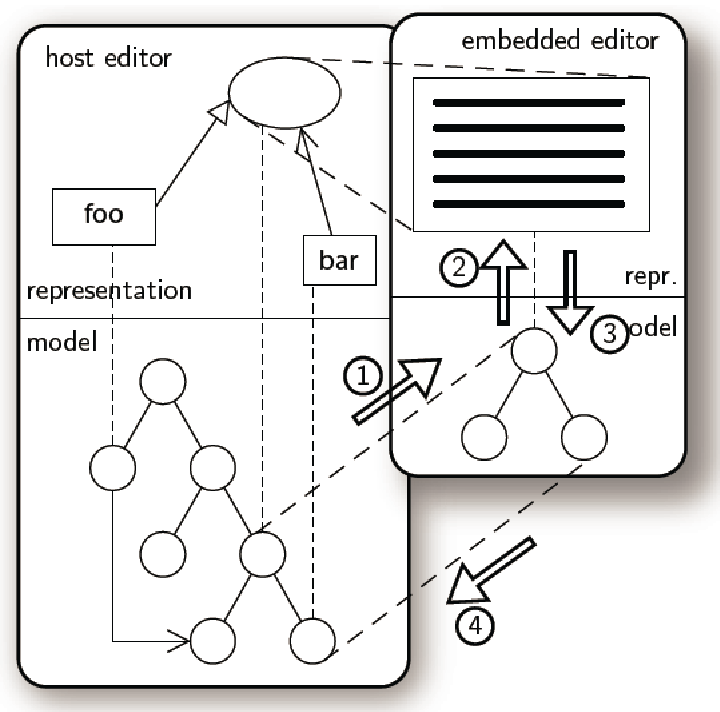
\includegraphics[scale=0.7]{gfx/tef.png}

Replacing has two fundamental problems:
\begin{itemize}
	\item all references to the replaced element break.
	\item Information which is contained in the orginal model, but not displayed in the textual representation is lost.
\end{itemize}
In order to solve the problems by reassigning the references and merging the models, identification is required. \cite{TefPaper} demands language-specific identification. 

TEF does not require the whole model to be describable textually, only the elements and it's directly or indirectly contained elements which should be textually displayable must be specified using a CFG.

TEF creates a Parse-tree from the model by traversing the model along its composition and determines a set of suitable grammar rules based on constraints. It uses backtracking for that and \cite{TefPaper} also suggest to enable the language engineer to prioritize grammar rules if multiple parse trees are possible.

\chapter{XText Architecture}
\label{cha:xtextarch}
This section describes how XText realizes the concepts described by the grammar. It focuses on Parsing, Unparsing, the gap between abstract syntax and parse tree, Referential Integrity. \todo{sounds like shit}

XText converts saves the input grammar as an EMF model and generates GrammarAccess methods, which are used at various points in the runtime. XText integrates itself in EMF as a Resource.  The basic components of a XText resources are the Serializer, to convert EObjects to text, the Parser, to convert text to EObjects or to deserialize the EObjects and the Linker which manages Cross-References. 
\todo{Bild einbinden}
\section{Parsing}
XText uses ANTLR\cite{ANTLR} for parser creation. It creates ANTLR grammar files with ANTLR Grammar Actions to create the AST and ParseTree. The rules return EObjects, 'init' and 'after' actions are used as guidance of the current stack position for the creation of nodes. The returned EObjects form the AST, but orthogonal to them, a node model is created which is related to the AST. 

\section{Node Model}
The node model is created during parsing. It is important to note, that the node model is not an EMF model. The base interface of the node model is INode which  is described as "A node in the parse tree"\cite{XTextAPI}. Nodes are either composite nodes if they represent non terminals or leaf nodes, if they represent terminals. Nodes hold a reference to the grammar element they represent and leafs to the represented token additionally. Nodes are added to the EObjects as Adapters.

The roles of the node model during serializations are:
\begin{itemize}
	\item preserves existing white spaces
	\item preserves existing comments
	\item preserves the representation of cross-references, in case multiple names are possible
	\item preserves the representation of values, in case multiple representations are possible, e.g. 1.0, 1.00, 1.000.
\end{itemize}

\section{Linking}
\label{sec:xtextarch:Linking}
Linking in XText can be separated into two parts:
\begin{itemize}
	\item how XText copes with the impedance mismatch between cross references and Xtext in general. In this case, just inner resource references are considered. 
	\item how does XText resources cope with integration in EMF as an EMF resource.
\end{itemize}
The general idea of linking in XText is that every grammar rule which contains a reference is visited after the ANTLR parser finished. While visiting the AST, an ILinker instance is consulted to resolve the link programmatically using the the links textual representation saved in the node model and the context, which is EObject holding the reference. XText strongly encourages the usage of a lazy linkers, which replaces the link with an EMF proxy containing the proper URI. This also solves the problem where links depend on each other automatically.

Beside the option to export just a subset of XTexts created EObjects, to achieve full EMF integration every EObject has to be referable, so the resource must be able to return the URI fragment of the given contained EObject and the EObject for a URI fragment. By default, XTexts Fragment Provider  uses path fragments like \kode{//@classes.0/@methods.0/@localVariables.3/@name}. XTexts documentation states that path references are fragile and that UUIDs should not be used regarding the users. 

\section{Concrete Syntax Validation Constraints}
As mentioned in \cite{MofCfg}, it is possible to create invalid metamodels, where no valid textual representation can be deduced, even if the metamodel was inferred from the EBNF. The validation constraints described constrain each grammar rule. They are not simply used to validate if a textual representation is possible, but are also used to guide the serialization process to distinguish between different production and grammar rules, e.g.
\begin{xtxt}
Z 	:  "A" v=ID  
	|  "B" n=INT;
\end{xtxt}
given an instance of 'Z', it depends on if 'v' or 'n' is assigned to properly serialize 'Z'.
Given the rule
\begin{xtxt}
MyRule:	({MySubRule} "sub")? (strVal+=ID intVal+=INT)*;
\end{xtxt}
several constraints are implied:
\begin{enumerate}
	\item types: just instances of MyRule and MySubRule are allowed. Because subtypes can't be created by the parser, they're prohibited. 
	\item Features: if other structural features besides strVal and intVal exist, they must be either transient, unassigned or contain the default value.
	\item Quantities: the size of strVal and intVal must be equal.
	\item Values: all values must be convertable to valid terminal tokens.
\end{enumerate}
These constraints are created per production rule, not only per grammar rule, in case of 'Z' two independent set of constraints are created.
XTexts concrete syntax validation is not capable of regarding:
\begin{enumerate}
	\item assigned actions, e.g. 
	\kode!{MyType.myFeature=current}!
	\item unassigned rule calls to assigned actions
	\item the order within list features, e.g. In \kode{Rule: (foo+=R1 foo+=R2)*} foo must contain R1 and R2 in alternating order
\end{enumerate}

\section{Serialization}
The serialization process complements parsing and lexing by transforming EMF models into its textual representation. The XText documentation mentions six relevant steps:

\begin{enumerate}
	\item Validation
	\item Matching model elements with grammar rules by the parse tree constructor
	\item Associating comments
	\item Associating existing nodes
	\item merge white spaces and line wraps
	\item adding white spaces by the formatter
\end{enumerate}

In this thesis, only the parse tree constructor is discussed because:
\begin{itemize}
	\item validation is optional and is done with less meaningful error messages by the parse tree constructor
	\item comments, white spaces, line wraps are layout information without grammar relation.
	\item Runtime analysis with breakpoints showed that the existing node model is already accessed by the parse tree constructor, which indicates a gap in documentation and implementation.
\end{itemize}

\subsection{The contract}
"The contract of serialization says that a model which is saved (serialized) to its textual representation and then loaded (parsed) again yields a new model that is equal to the original model."\cite{XTextMan}

in short:\\
I) $load(save(model)) \rightarrow model$\\
The inverse does not always hold, thus:\\
II) $save(load(text)) \nrightarrow text$\\
If the node model still exists, II) holds in most cases. 

Given the XText example, that for the rule
\begin{xtxt}
MyRule: (xval+=ID | yval+=INT)*; 
\end{xtxt}
first all xvals and then all yvals will be written to the token stream indicates that XText follows the  EObject containment order instead of the one of the node model.

\subsection{Parse Tree Constructor}  \label{xtxt:ptc}
Actually the ParseTree constructor (PTC) does not construct nodes of the node model, it just finds valid grammar rules for each EObject of the AST. It succeeds if all EObjects are visited and no concrete syntax validation constraint is violated. So the PTC has to find a valid allocation for the traversed AST in which all grammar constraints hold.  This is, like parsing, a constraint satisfaction problem (CSP). XText solves this CSP  using top down backtracking, which results in exponential runtime of the serialization of a model. This is done by PTC finding valid 'paths' from the root to a leaf node constrained by the grammar. The PTC does The PTC stops after the first valid solution has been found. 

For example, if the following grammar parses \kode{somekeyword 0 C}:
\begin{xtxt}
S  	:  	v=A 
	| 	v=X;

A returns Obj	: 	l=B r=C   ;
X returns Obj	: 	l=Y r=Z   ;
B returns N  	:  	"somekeyword" 	v="0";
Y returns N  	: 	"otherkeyword" 	v="0";
C 		:  	 "C" ;
Z 		: 	 "Z" ;
\end{xtxt}
following AST will be constructed \todo{fix this} \\ 
      Obj			\\
     /   \textbackslash		\\
N(v='0')   C	\\
To unparse the this parse tree without a node model, the decision if the rule of the root EObject is 'A' or 'X' can just be decided after determining the type of it's right child 'C'. \\

It is possible that all grammar rules return the same type, so type information would be useless to guide production rule resolution.\\
Furthermore, if there is no representation of a choice in the AST, a default needs to be specified, for example in the case: 
\begin{xtxt}
PluralRule: "contents:" count=INT Plural;
terminal Plural: "item" | "items";
\end{xtxt}
it is unclear during unparsing if 'item' or 'items' should be used. This case is named unassigned text in XText.

\subsection{Xtext Implementation as EMF  Resource}
XText is integrated in EMF as a resource, XTextResource.\\
The main drawbacks of this solution are:
\begin{itemize}
	\item During incremental changes, the XText parser replaces subtrees instead of updating them, so existing EObjects become stale. The XText documentation advices against the use of a "self-synchronizing (...) editor" on the same model as XText but suggests working on a copy.
	\item The implementation to identify EObject in a resource has to return stable fragments.
\end{itemize}

\section{Review / Criticism}
\subsection{XText Grammar}
The XText grammar still leaves room for improvement. It is not possible do statically assign a value  to a structural feature. For example assigning 0 to an integer attribute 'v' of class MyBoolean in the "false" case and 1 in the "true" case requires to write a special value converter. 
\begin{xtxt}
MyBoolean:  "true" | "false"
\end{xtxt}

A much greater impact on the grammar is it's inability to express left recursive grammars and the consequences. This is owed to the LL(*) parsing algorithm which is used by parser generator ANTLR used by XText to create the parser. This requires left factoring and grammar rewriting which forces XText to allow assigned actions, thus tree rewriting of the AST. If only parser and AST construction is regarded, this is more or less an inconvenience for the grammar designer, but it creates problems regarding unparsing and validation for XTexts current implementation. Considering that the current unparsing algorithm has $O(exp(n))$ it is arguable to use an GLR parsing algorithms with  $O(n^3)$ to avoid the need for grammar massaging and thus AST rewriting.

\subsection{XText Resource}
XText is, like EMFTex \cite{EMFTextMan}, only integrated in EMF as an EMF Resource. Because the responsibility of resources are to serialize and deserialize models., this is the origin of various problems: 

\begin{itemize}
	\item The grammar must describe the whole model: the model must not contain non volatile information which is not regarded by the grammar and adding additional information, like an ID, is impossible without incorporating it in the grammar. To circumvent the restriction that the whole model must be textually described, a possible solution would be to create additional EObjects in an extra Resource pointing at the to be extended EObject in a XTextResource with a CrossReferenceAdapter and requesting the inverse references of  the extended object. This technique to extend an EObject in a non invasive manner is used to implement UML2 stereotypes in eclipse UML. This concept depends on references and their integrity.
	\item The XText editor edits the text file, meaning it edits the serialized form of the model, not the model. As a result, model elements are replaced instead of updated. Furthermore, EMFs ResourceSet which keeps referential integrity is bypassed. XTexts demands the programmer to handle referential integrity or to "return stable fragments for its contained elements ". For example the expression "int i=0" in a programming language does not contain an intrinsic identifier, so this is impossible for an arbitrary language. UML2 solves the problem of referential integrity by assigning every model element an universal unique identifier (UUID). These UUIDs are handled by the resource and are  externally attached to the model objects. To keep referential integrity, either modifications must be done in a ResourceSet or extrinsic UUIDs must be used. 
	\item Because the model contained in a resource is not modified in a ResourceSet and extrinsic, non grammar conform information like IDs can't be added or integrated persistently to model elements referential integrity can not be maintained. On the other hand to determine changes to update a model without unique IDs must inevitable  be based on heuristics, thus being inaccurate.  To enable proper updates and keep referential integrity, editing must not be done on the textual serialized form of a model. This does not contradict to store the model in textual form for e.g. viewing and versioning. 
\end{itemize}

\subsection{Node Model}
The potential use of the node model is strongly restricted in Xtext, for the following reasons:
\begin{itemize}
	\item the node model is not an EMF model. 
	\item The node model is not explicitly available without running the XText parser, because it is created at runtime from the information available from the serialized language model implementation. 
	\item The use of the runtime instances of the node model is strongly restricted by the API: ``clients should never keep a reference to a node as it may be invalidated at any time and the very same object could be reused in another subtree of the full parse tree.''\cite{XTextAPI}
	\item The node model is not updated during unparsing, but an additional parse with its associated update behavior is necessary.
	\item Even if the PTC would construct the node model, it takes the first valid solution. It is not possible to choose between different valid representations or prefer a valid one which are semantically equivalent, e.g.\begin{xtxt}
Foreach 		: 	Map | For;
Map returns FE  	:  	"map" 		v=ID;
For returns FE  	: 	"foreach"	v=ID;
\end{xtxt}
\end{itemize}